%----------------
\begin{figure*}
  \centering
  \subfloat[\covtype]{
  \centering 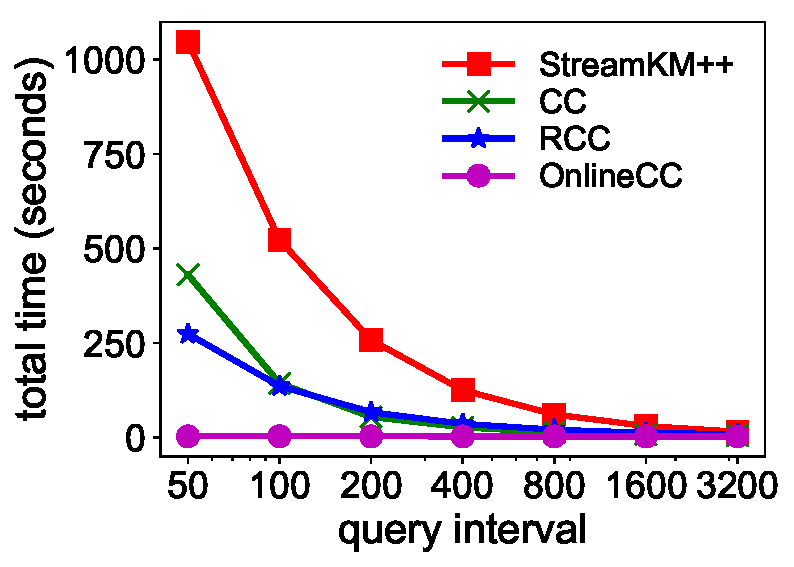
\includegraphics[width=0.23\textwidth]{expfigs/totaltime_q/covtype_total_vs_q.pdf}
  }
  \subfloat[\power]{
  \centering 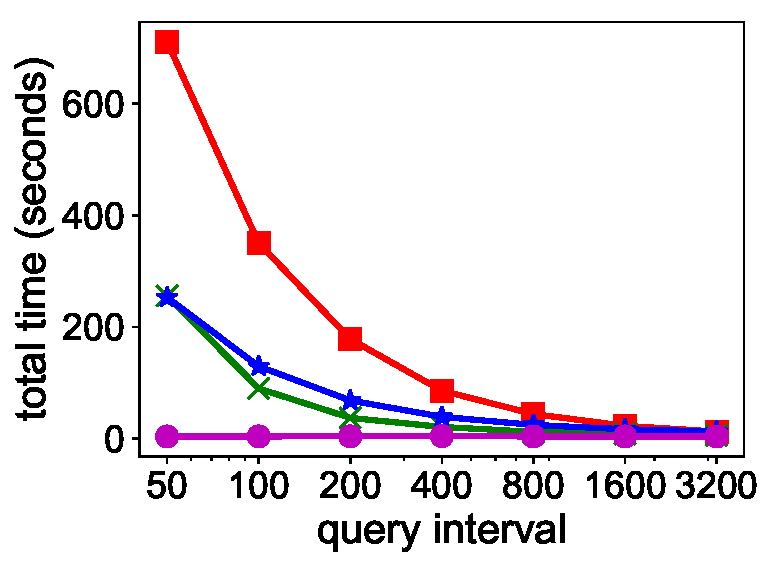
\includegraphics[width=0.23\textwidth]{expfigs/totaltime_q/power_total_vs_q.pdf}
  }
  \subfloat[\intrusion]{
  \centering 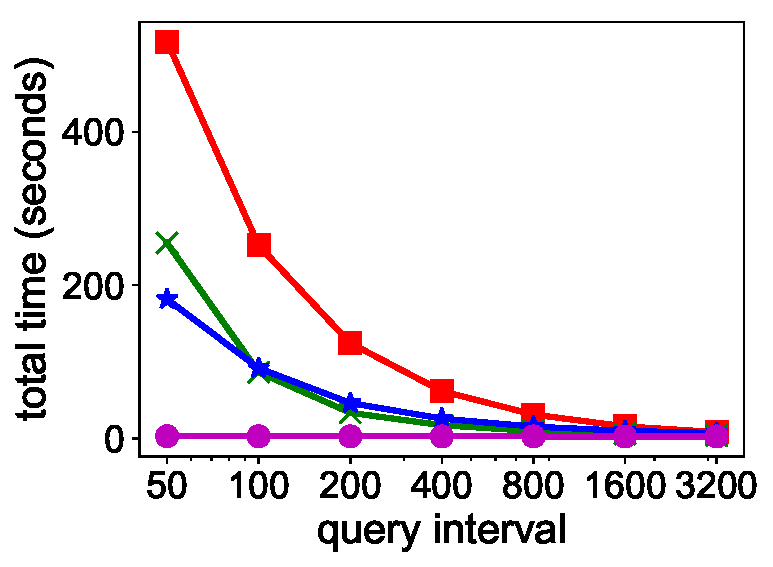
\includegraphics[width=0.23\textwidth]{expfigs/totaltime_q/intrusion_total_vs_q.pdf}
  }
  \subfloat[\drift]{
  \centering 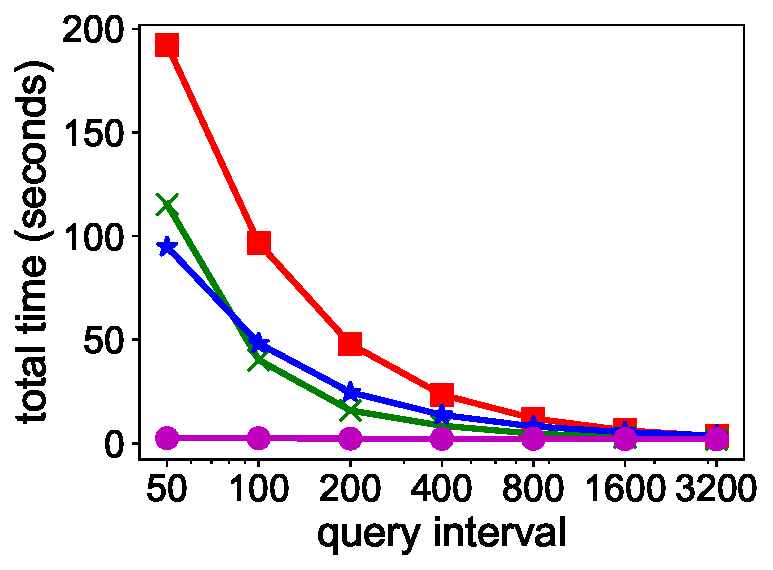
\includegraphics[width=0.23\textwidth]{expfigs/totaltime_q/synthetic_total_vs_q.pdf}
  }
  \caption{Total time (seconds) vs. query interval $q$. The total time is for the entire dataset overall stream. For every $q$ points, there is a query for the cluster centers. The number of centers $k$ is $30$.}
 \label{fig:time-versus-q}
\end{figure*}
%----------------